\documentclass[11pt]{beamer}
\usetheme{Madrid}
\usepackage[utf8]{inputenc}
\usepackage[english]{babel}
\usepackage{amsmath}
\usepackage{amsfonts}
\usepackage{amssymb}
\usepackage{graphicx}
\def\gint{\displaystyle\int}

\author[Matthieu Brachet]{M. Brachet}
\title[Journées EDP]{Numerical approximation using a compact scheme for evolution problems on the sphere}
\institute[IECL]{Institut Elie Cartan de Lorraine,\newline UMR CNRS 7502, Dép. de Mathématiques,\newline Metz, France} 
\date{March 30th, 2017} 

\begin{document}

\begin{frame}
\titlepage
\includegraphics[scale=0.22]{iecl.jpg}
\includegraphics[scale=0.41]{ul.jpg}
\end{frame}

\begin{frame}{}
\begin{itemize}
\item Works at Institut Elie Cartan de Lorraine (Metz, France),
\item PhD supervised by Jean-Pierre Croisille.
\end{itemize}
\end{frame}

%% ***************************************************************************************************************************************

\begin{frame}{Motivations}
\begin{block}{PDEs problems on the sphere $\mathbb{S}^2_R$}
Atmosphere and ocean: complex PDEs on the sphere occur in climatology, oceanology, ...
\end{block}

\begin{block}{Approximating PDE on the Sphere}
\begin{itemize}
\item Analytic solution are not available in general,
\item Approximated solutions are required.
\end{itemize}
\end{block}
\end{frame}


\begin{frame}{Outline}
\begin{enumerate}
\item The Cubed-Sphere
\item Differential operators on the Cubed-Sphere
\item Hermitian scheme on the Cubed-Sphere
\item Numericals results.
\end{enumerate}
\end{frame}


\begin{frame}{Example : latitude/longitude grid}
\begin{columns}
\column{0.35\textwidth}
\begin{itemize}
 \item $\lambda$ : longitude angle,
 \item $\theta$ : latitude angle.
\end{itemize}

\column{0.65\textwidth}
\begin{center}
\begin{figure}
\includegraphics[scale=0.2]{latlon.png}
\caption{Longitude-Latitude coordinates}
\end{figure}
\end{center}
\end{columns}
\end{frame}


\begin{frame}{The Cubed-Sphere}
\begin{columns}
\column{0.45\textwidth}
\begin{figure}
   \def\svgwidth{1 \textwidth}
\input{drawing12.pdf_tex}
\end{figure}

\column{0.45\textwidth}
\begin{itemize}
\item Idea : two sets of intersecting great circles,
\item The Cubed-Sphere use points of intersection,
\item This grid was introduced by R. Sadourny in 1972.
\end{itemize}
\end{columns}
\end{frame}



\begin{frame}{Definition of grid points}
\begin{block}{Definition of the Cubed-Sphere}
\begin{itemize}
\item The points of the Cubed-Sphere are intersects of two set of circles.
\item The circles in {\sl vertical} position are labeled $C^{(1)}_i$, $-N/2 \leq i\leq N/2$.
\item The circles in {\sl horizontal} position are labeled 
$C^{(2)}_j$, $-N/2 \leq j\leq N/2$.
\end{itemize}
\end{block}

\begin{block}{$C^{(1)}_i$ non orthogonal to $C^{(2)}_j$in general}
\begin{itemize}
\item Only the two circles in the center intersect orthogonally. 
\item A {\sl panel} is the squared region limitated by the two sets of circles. 
\end{itemize}
\end{block}
\end{frame}



\begin{frame}{Cubed-Sphere : 6 panels on the Sphere}
\begin{block}{Panel with parameter $N=8$}
\begin{columns}
\column{0.55\textwidth}
$N^2$ is the number of cells in a panel. 

The gridpoints are classified in three categories :
\begin{itemize}
\item RED CIRCLES = {\sl internal} points,
\item BLUE SQUARES = {\sl edge} points,
\item YELLOW PENTAGONS = {\sl corner} points.
\end{itemize}

\column{0.45\textwidth}
\begin{figure}
   \def\svgwidth{1 \textwidth}
\input{drawing13.pdf_tex}
\end{figure}
\end{columns}
\end{block}
\end{frame}


\begin{frame}{The Cubed Sphere grid}
\begin{figure}
\begin{center}
\hspace{-1.cm}
\includegraphics[scale=0.3]{plot_CS.png}
\caption{\footnotesize
The Cubed-Sphere grid with $N=16$.
}
\end{center}
\label{fig:1.4}
\end{figure}
\end{frame}


\begin{frame}{Coordinate angles on panel (I) (=Frontal panel)}
\begin{block}{Angles $\xi$ and $\eta$}
On each pannel the local coordinate system
consists of :
\begin{itemize}
\item the \textbf{first equatorial angle} $\xi$ with $-\pi/4 \leq \xi \leq \pi/4$ (zonal),
\item the \textbf{second equatorial angle} $\eta$ with $-\pi/4 \leq \eta \leq \pi/4$ (meridional).
\end{itemize}

\end{block}
\begin{figure}
\begin{center}
\includegraphics[scale=0.25]{face_cube4.jpg}
\caption{\footnotesize
$\bullet$ \textbf{Left:} Regular cartesian grid using $(\xi_F,\eta_F)$ coordinates of the panel (I),\newline
$\bullet$ \textbf{Right:} Projection of the Grid onto the (I) face of the cube in the plane $x=1$.
}
\label{fig:1}
\end{center}
\end{figure}
\end{frame}


\begin{frame}{Local basis}
\begin{block}{Six local non-orthogonal coordinate systems}
The cubed-sphere consists of six panels with number $(k)=(I),(II),\dots, (VI)$
with coordinates $(\xi^{(k)}, \eta^{(k)})$.
\end{block}
\begin{block}{Canonical local basis in a panel}
The local basis at $\mathbf{x} \in \mathbb{S}^2_R$ is
\begin{equation}
\mathbf{x} \in \mathbb{S}^2_R \mapsto (\mathbf{g}_\xi(\mathbf{x}),\mathbf{g}_\eta(\mathbf{x}))
=(\partial_\xi \mathbf{x}, \partial_\eta \mathbf{x}) \in \mathbb{T}\mathbb{S}^2_R
\end{equation}
\end{block}
\begin{block}{Metric tensor $G$ }
The metric tensor at $\mathbf{x} \in \mathbb{S}_R^2$ is :
\begin{equation}
\label{eq:1001.3}
G=\left[ \begin{array}{cc}
\mathbf{g}_{\xi} \cdot \mathbf{g}_{\xi} & \mathbf{g}_{\xi} \cdot \mathbf{g}_{\eta} \\
\mathbf{g}_{\eta} \cdot \mathbf{g}_{\xi} & \mathbf{g}_{\eta} \cdot \mathbf{g}_{\eta} \\
\end{array} \right] 
\end{equation}
\end{block}
\end{frame}


\begin{frame}{Dual basis}
\begin{block}{Dual basis}
\begin{itemize}
\item The dual basis at $\mathbf{x} \in \mathbb{S}^2_R $ is $(\mathbf{g}^\xi(\mathbf{x}),\mathbf{g}^\eta(\mathbf{x}))$ ("contravariant basis") is related to $(\mathbf{g}_\xi,\mathbf{g}_\eta)$ by:
$
\left\{
\begin{array}{c}
\mathbf{g}^\xi=G^{11} \mathbf{g}_\xi+G^{12} \mathbf{g}_\eta,\\
\mathbf{g}^\eta=G^{21} \mathbf{g}_\xi+G^{22} \mathbf{g}_\eta
\end{array}
\right.
$

where
\begin{equation}
G^{-1}=
\left[
\begin{array}{cc}
G^{11}& G^{12}\\
G^{21}& G^{22}
\end{array}
\right]
\end{equation}
\end{itemize}
\end{block}

\begin{block}{Example : expression on panel (I)}
The dual basis $(\mathbf{g}^\xi, \mathbf{g}^\eta)$ is expressed in coordinates $x,y,z$ by :
\begin{equation}
\label{eq:1001.4}
\mathbf{g}^\xi=
\frac{1}{x(1+X^2)} \left[
\begin{array}{c}
-X\\
1\\
0
\end{array}
\right]
,\;\;\;
\mathbf{g}^\eta=
\frac{1}{x(1+Y^2)} \left[
\begin{array}{c}
-Y\\
0\\
1
\end{array}
\right]
\end{equation}
where $X = y/x$ and $Y = z/x$.
\end{block}
\end{frame}

\begin{frame}{Gradient, Divergence and Curl}

\begin{block}{Differential operators}
Let $\mathbf{u} : \mathbb{S}_R^2 \mapsto \mathbb{T}\mathbb{S}_R^2$ and $h : \mathbb{S}_R^2 \mapsto \mathbb{R}$ be regular functions. Then :
\begin{itemize}
\item Gradient :
\begin{equation}
\nabla_T h = \dfrac{\partial h}{\partial \xi} \mathbf{g}^{\xi} + \dfrac{\partial h}{\partial \eta} \mathbf{g}^{\eta}
\end{equation}
\item Divergence :
\begin{equation}
\nabla_T \cdot \mathbf{u} = \dfrac{\partial \mathbf{u}}{\partial \xi}\cdot \mathbf{g}^{\xi} + \dfrac{\partial \mathbf{u}}{\partial \eta} \cdot \mathbf{g}^{\eta}
\end{equation}\\
\item Curl :
\begin{equation}
\nabla_T \wedge \mathbf{u} = \dfrac{\partial \mathbf{u}}{\partial \xi}\wedge \mathbf{g}^{\xi} + \dfrac{\partial \mathbf{u}}{\partial \eta} \wedge \mathbf{g}^{\eta}
\end{equation}

\end{itemize}

\end{block}
\end{frame}

%% ***************************************************************************************************************************************

\begin{frame}{Grid function on the Cubed-Sphere}

\begin{block}{Discrete data representation}
A set of data at Cubed-Sphere points is called a \textbf{grid function}.
\end{block}

\begin{block}{Grid function}
A grid function on the Cubed-Sphere consists of the 6
sets of data
\begin{equation}
u^k_{i,j},\;\; -N/2 \leq i,j\leq N/2,\;\; k\in\lbrace (I),(II),(III),(IV),(V),(VI) \rbrace,
\end{equation}
\end{block}
\begin{block}{Spherical periodicity}
The spherical periodicity is expressed as 
\begin{itemize}
\item Matching the values along the 12 edges.
\item Matching the values at the 8 corners.
\end{itemize}
\end{block}
\end{frame}

\begin{frame}{Three-point Hermitian Derivative Operator}

\begin{block}{Local formula : }
Standard local finite difference scheme of a sequence $(u_j)_{j \in \mathbb{Z}}$ :
\begin{equation}
\dfrac{u_{j+1}-u_{j-1}}{2\Delta x} = \delta_x u_j \;\;\; j \in \mathbb{Z}
\end{equation}
\end{block}

\begin{block}{Second order accuracy}
Approximation of $u'(x_j)$ :
\begin{equation}
\delta_x u_j = u'(x_j) + \dfrac{1}{12} \partial_x^{(3)} u(x_j) \Delta x^2 + \mathcal{O}(\Delta x^4)
\end{equation}
\end{block}


\end{frame}

\begin{frame}{Truncation error of Hermitian derivatives}
\begin{block}{Non-local finite difference derivative}
The standard {\bf Hermitian discrete derivative} of a sequence 
$(u_j)_{j \in \mathbb{Z}}$ is 
the sequence $(u_{x,j})_{j \in \Bbb Z}$ defined by
\begin{equation}
\sigma_x u_{x,j}=\delta_x u_j,\;\; j \in \mathbb{Z},
\end{equation}

where
$\sigma_x$, $\delta_x$ are the finite difference operators
\begin{equation}
\underbrace{\frac{1}{6}u_{x,j-1}+\frac{2}{3}u_{x,j}+\frac{1}{6}u_{x,j+1}}_{\sigma_x u_{x,j}} 
= 
\underbrace{{ u_{j+1}-u_{j-1} \over 2 \Delta x}}_{\delta_x u_j},\;\; \Delta x >0
\end{equation}

\end{block}

\begin{block}{Fourth-order accurate formula}
The Hermitian derivative is pointwise fourth-order accurate:
\begin{equation}
u_{x,j}=u^\prime(x_j)-\frac{1}{180}\partial_x^{(5)} u(x_j)\Delta x^4+O(\Delta x^6)
\end{equation}
\end{block}


\end{frame}

\begin{frame}{Good representation of high frequencies}
\begin{itemize}
\item If $u(x)=e^{i x \xi}$, then $u'(x)=i \xi u(x)$,
\item $u_{x,j} = \dfrac{i}{\Delta x} \theta_m ( \Delta x \xi ) u(x_j)$ is the discrete derivative,
\item $
\begin{array}{rcl}
u'(x_j) - u_{x,j} & = & \dfrac{i}{\Delta x} \left( \Delta x \xi - \theta_m(\Delta x \xi) \right) u(x_j)
\end{array}
$
\end{itemize}

\begin{columns}
\column{0.45\textwidth}
\begin{block}{Accuracy}
\begin{itemize}
\item Consistency :
$$
\theta_m ( \Delta x \xi ) - \Delta x \xi \approx 0
$$
\item The compact approximation is well known for its very good accuracy.
\end{itemize}
\end{block}

\column{0.45\textwidth}
\begin{center}
\begin{figure}
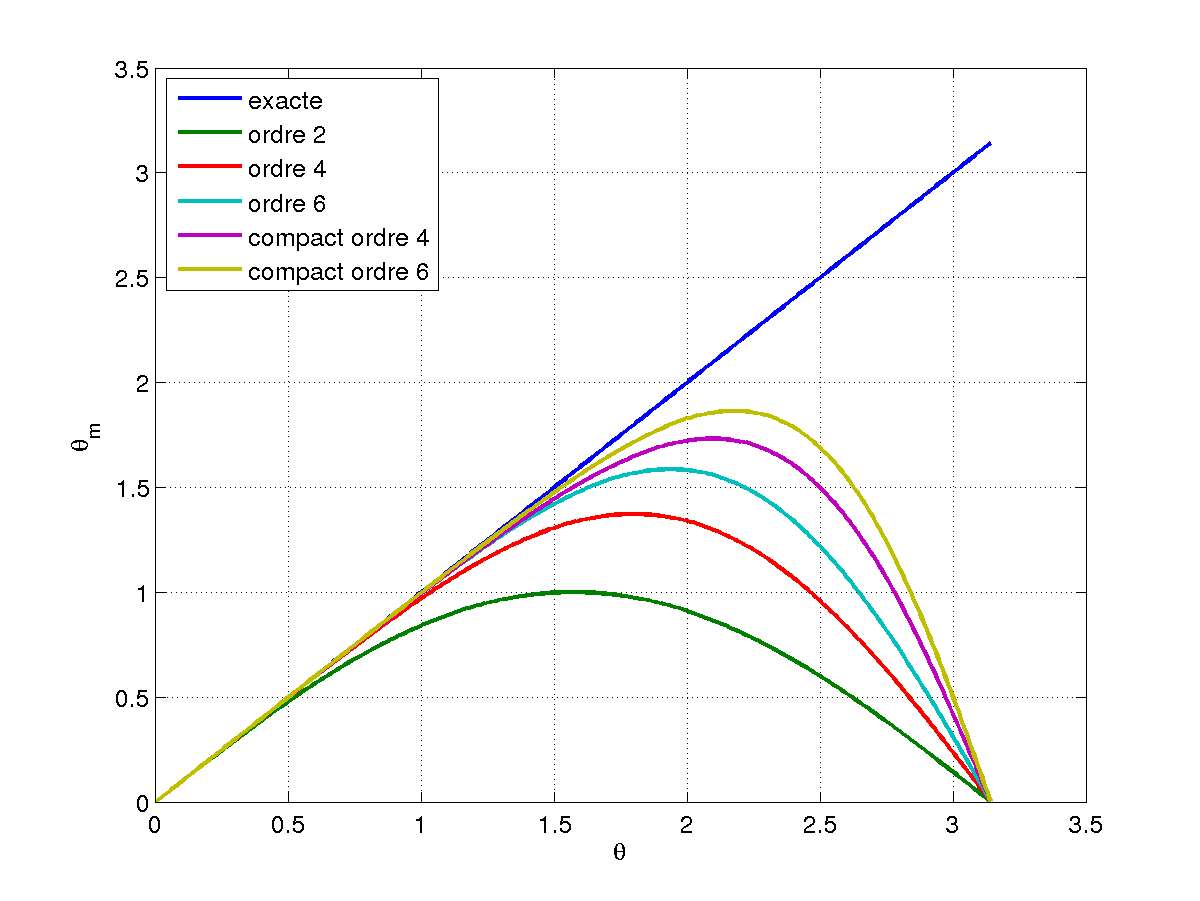
\includegraphics[scale=0.4]{onde_modifiee.png}
\end{figure}
\end{center}
\end{columns}
\end{frame}

%% ***************************************************************************************************************************************

\begin{frame}{Discrete operators on the Cubed-Sphere}
\begin{itemize}
\item Data along any great circle on the sphere can be differentiated by a compact well chosen scheme.
\item At each grid point, two great cicles are intersecting. 
\item Reconstruct an approximate differential operator from a set of suitable selected Hermitian derivatives .
\end{itemize}
\end{frame}


\begin{frame}{Principe of interpolating data along great circles}
\begin{figure}
\begin{center}
\includegraphics[scale=0.15]{fig35.jpg}
\label{fig:152}
\end{center}
\end{figure}
\begin{itemize}
\item Panels (I) and (III) : simple copy of data.
\item Panels (II) and (IV): interpolation data using cubic splines along iso-$\xi$ lines.
\end{itemize}
\end{frame}

\begin{frame}{Discrete differential operators}

$\Delta = (\Delta \xi, \Delta \eta)$ represents the discrete parameter.

\begin{block}{Discrete gradient, divergence and curl}
on panels (I) and (III) using
\begin{equation}
\nabla_{T}h=\frac{\partial h}{\partial\xi}_{|\eta}\mathbf{g}^{\xi}
+\frac{\partial h}{\partial\eta}_{|\xi}\mathbf{g}^{\eta} \approx \nabla_{T,\Delta} h=h_{\xi}\mathbf{g}^{\xi}
+h_{\eta} \mathbf{g}^{\eta}
\end{equation}
\begin{equation}
\nabla_{T} \cdot \mathbf{u}=\frac{\partial \mathbf{u}}{\partial\xi}_{|\eta} \cdot \mathbf{g}^{\xi}
+\frac{\partial \mathbf{u}}{\partial\eta}_{|\xi} \cdot \mathbf{g}^{\eta} \approx \nabla_{T,\Delta} \cdot \mathbf{u}=\mathbf{u}_{\xi} \cdot \mathbf{g}^{\xi}
+\mathbf{u}_{\eta} \cdot \mathbf{g}^{\eta}
\end{equation}
\begin{equation}
\nabla_{T} \wedge \mathbf{u}=\frac{\partial \mathbf{u}}{\partial\xi}_{|\eta} \wedge \mathbf{g}^{\xi}
+\frac{\partial \mathbf{u}}{\partial\eta}_{|\xi} \wedge \mathbf{g}^{\eta} \approx \nabla_{T,\Delta} \wedge \mathbf{u}=\mathbf{u}_{\xi} \wedge \mathbf{g}^{\xi}
+\mathbf{u}_{\eta} \wedge \mathbf{g}^{\eta}
\end{equation}
where $(\mathbf{g}^{\xi},\mathbf{g}^{\eta})$ is the dual basis at $(\xi,\eta)$ and $h_{\xi}$, $h_{\eta}$, $\mathbf{u}_{\xi}$ and $\mathbf{u}_{\eta}$ are Hermitian derivatives.
\end{block}
\end{frame}


\begin{frame}{Discrete differential operators}
\begin{block}{Proposition :}
Let $h:\mathbb{S}^2 \mapsto \mathbb{R}$ and $\mathbf{u}: \mathbb{S}^2 \mapsto \mathbb{T}\mathbb{S}^2$ be regular functions. Then:

\begin{itemize}
\item Gradient : \begin{equation}
\| (\nabla_{T}h)^* - \nabla_{T,\Delta}h^* \|_{\infty} \leq \mathcal{O} \left( \Delta \xi^3, \Delta \eta^3 \right)
\end{equation}

\item Divergence : \begin{equation}
\| (\nabla_{T}\cdot \mathbf{u})^* - \nabla_{T,\Delta}\cdot \mathbf{u}^* \|_{\infty} \leq \mathcal{O} \left( \Delta \xi^3, \Delta \eta^3 \right) 
\end{equation}

\item Curls : \begin{equation}
\| (\nabla_{T}\wedge \mathbf{u})^* - \nabla_{T,\Delta}\wedge \mathbf{u}^* \|_{\infty}  \leq  \mathcal{O} \left( \Delta \xi^3, \Delta \eta^3 \right)
\end{equation}
\end{itemize}
$\cdot^*$ means "restricted to the grid.
\end{block}

\begin{block}{Effective order accuracy}
In pratice, fourth order is observed for the three cases!
\end{block}
\end{frame}
%
%\begin{frame}{Test 1: Accuracy of the calculated gradient}
%\begin{block}{Approximate gradient of $u(x,y,z)=\sin(10\pi x)\sin(2\pi y)\sin(6\pi z)$}
%\tiny
%\begin{table}[h!]
%\begin{center}
%\begin{tabular}{|c||c|c|c|c|c|c|c|}
%\hline 
% & N=16 & rate & N=32 & rate & N=64 & rate & N=128\\
%\hline
%\hline 
%$e_\infty$ &  1.912(-5) & 4.00 & 1.191(-6) & 4.00 & 7.432(-6) & 3.72 & 5.622(-9)\\
%\hline 
%$\Delta \xi$ in km &  625 &  & 312.5 &  & 156.25 &  & 78.12\\
%\hline
%Nb of grid points &  1538 &  & 6146 &  & 24578 &  & 93306\\
%\hline
%\end{tabular}
%\vspace{0.2cm}
%\caption{\footnotesize Convergence rate of the hermitian gradient of the oscillating 
%function $u(x,y,z)=\sin(10\pi x)\sin(2\pi y)\sin(6\pi z)$
%restricted to the unit sphere.}
%\label{table:2}
%\end{center}
%\end{table}
%\normalsize
%\end{block}
%\end{frame}
%
%
%\begin{frame}{Test 3: Accuracy of the calculated divergence}
%\begin{block}{Approximate divergence of $\mathbf{F}(\mathbf{x}) = c(\mathbf{x}) \mathbf{n}(\mathbf{x}) \times \mathbf{\psi}(\mathbf{x})$}
%
%with $c(\mathbf{x}) \mathbf{\psi}(\mathbf{x}) = \sin (2 \pi x ) \sin( 6 \pi y) sin(10 \pi z ) \begin{pmatrix}
%1\\2\\3
%\end{pmatrix}$.
%\tiny
%\begin{table}[h!]
%\begin{center}
%\begin{tabular}{|c||c|c|c|c|c|c|c|}
%\hline 
% & N=16 & rate & N=32 & rate & N=64 & rate & N=128 \\
%\hline
%\hline 
%$e_\infty$         & 5.3116 (-1) & 4.5098 & 2.3315 (-2) & 4.2859 & 1.1952 (-3) & 4.0891 & 7.0225 (-5) \\
%$\Delta \xi$ in km & 625         &        & 312.5       &        & 156.25      &        & 78.12       \\
%Nb of grid points  & 1538        &        & 6146        &        & 24578       &        & 93306       \\
%\hline
%\end{tabular}
%\vspace{0.2cm}
%\caption{\footnotesize Convergence rate of the hermitian divergence of  $\mathbf{F}(\mathbf{x}) = c(\mathbf{x}) \mathbf{n}(\mathbf{x}) \times \mathbf{\psi}(\mathbf{x})$ restricted to the unit sphere.}
%\label{table:2}
%\end{center}
%\end{table}
%\normalsize
%\end{block}
%\end{frame}

%\begin{frame}{Example : accuracy of the calculated curl}
%\begin{block}{Approximate curl of the tangential vector field $\mathbf{u} = u(\theta) \mathbf{e}_{\lambda}$}
%\tiny
%with $u(\theta)=\left\lbrace
%\begin{array}{ll}
%\dfrac{80}{e_n} exp\left( \dfrac{1}{(\theta-\theta_0)(\theta-\theta_1)} \right) & \text{ if } \theta_0 \leq \theta \leq \theta_1 \\
%0 & \text{ else}
%\end{array}\right.$ with $e_n$ a normalization constant.
%\begin{table}[h!]
%\begin{center}
%\begin{tabular}{|c||c|c|c|c|c|c|c|}
%\hline 
% & N=16 & rate & N=32 & rate & N=64 & rate & N=128 \\
%\hline
%\hline 
%$e_\infty$         & 4.4750 (-2) & 2.9553 & 5.7696 (-3) & 4.0753 & 3.4225 (-4) & 4.3341 & 1.6969 (-5) \\
%$\Delta \xi$ in km & 625         &        & 312.5       &        & 156.25      &        & 78.12       \\
%Nb of grid points  & 1538        &        & 6146        &        & 24578       &        & 93306       \\
%\hline
%\end{tabular}
%\vspace{0.2cm}
%\caption{\footnotesize Convergence rate of the Hermitian curl of the zonal 
%function $\mathbf{u} = u(\theta) \mathbf{e}_{\lambda}$
%restricted to the sphere.}
%\label{table:2}
%\end{center}
%\end{table}
%\normalsize
%\end{block}
%\end{frame}

\begin{frame}{Numerical order of accuracy of approximated curl}
\begin{block}{Approximate curl of a tangential vector field $\mathbf{u} = u(\theta) \mathbf{e}_{\lambda}$ (zonal dependance)}
$u(\theta)=\left\lbrace
\begin{array}{ll}
\frac{80}{e_n} \exp\left[ \frac{1}{(\theta-\theta_0)(\theta-\theta_1)} \right] & \text{ if } \theta_0 \leq \theta \leq \theta_1 \\
0 & \text{ else}
\end{array}\right.$ 

with $e_n$ a normalization constant.
\begin{figure}
\includegraphics[scale=0.35]{rate_vort.png}
\caption{\footnotesize Convergence rate of the Hermitian curl of the zonal 
velocity $\mathbf{u} = u(\theta) \mathbf{e}_{\lambda}$.}
\end{figure}
\end{block}
\end{frame}


\begin{frame}{Interest of the present approach}
\begin{block}{Advantage}
\begin{itemize}
\item Convergence rate: close to 4.
\item Easy change to alternative Hermitian formula due to the periodicity.
\end{itemize}
\end{block}

\begin{block}{Disadvantage}
\begin{itemize}
\item Redundant calculation : $24N^2$ Hermitian evaluations for $12N^2$ unknown,
\item Non-local calculation.
\end{itemize}
\end{block}
\end{frame}



%% *********************************************************************************************************************************

\begin{frame}{Advection equation}

\begin{block}{Advection equation}
\begin{itemize}
\item Let $\mathbf{c}:(\mathbf{x},t) \mapsto \mathbf{c}(\mathbf{x},t) \in \mathbb{T}\mathbb{S}_R^2$ a tangential vector field.
\item Find $h$ such that:
\begin{equation}
\left\lbrace
\begin{array}{rcl}
\dfrac{\partial h}{\partial t} + \mathbf{c} \cdot \nabla_{T} h & = & 0 \\
h(t=0,\mathbf{x}) & = & h_0(\mathbf{x}) 
\end{array}
\right.
\text{ on the sphere }  \mathbb{S}_R^2 \text{ for all } t>0.
\label{eq: advection}
\end{equation}
\end{itemize}
\end{block}
\end{frame}


\begin{frame}{Solid Body Rotation [Williamson and al., 1992]}
$\bullet$ $(\lambda, \theta)$ : longitude and latitude for $(NS)$ axis,

$\bullet$ $(\lambda', \theta')$ : longitude, latitude (axis $(NS)$ rotated by an angle $\alpha$).

\begin{columns}
\column{0.45\textwidth}
\begin{figure}
\def\svgwidth{0.6 \textwidth}
\vspace{0.5cm}
\input{drawing34.pdf_tex}
\end{figure}
\column{0.45\textwidth}
\begin{block}{}
\begin{equation*}
\left \{
\begin{array}{l}
\dfrac{\partial h}{\partial t} + \mathbf{c} \left( \mathbf{x} \right) \cdot \nabla_T h = 0\\[6pt]
h(0,\mathbf{x}) = h_0(\mathbf{x})\\
\end{array}
\right.
\end{equation*}

with $\mathbf{c} \left( \lambda', \theta' \right) = \omega_0  cos \theta' \mathbf{e}_{\lambda'}$.
\end{block}
\end{columns}

\begin{block}{}
Solution :
$$h \left( \mathbf{x} , t \right) = h_0 \left( R_{\omega_0 t}^{-1} \mathbf{x} \right)$$
with $R_{\theta}$ rotation matrix with angle $\theta$.

\end{block}
\end{frame}


\begin{frame}{Numericals observations}
\begin{columns}
\column{0.3\textwidth}
$\bullet$ Dispersive scheme
\begin{figure}
\href{run:ref_7363895058_test_0.avi}{\includegraphics[scale=0.1]{img_bump.png}} 
\end{figure}

\column{0.3\textwidth}
$\bullet$ Dissipative scheme
\begin{figure}
\href{run:ref_7363895782_test_0.avi}{\includegraphics[scale=0.1]{img_bump.png}} 
\end{figure}

\column{0.3\textwidth}
$\bullet$ Correct scheme
\begin{figure}
\href{run:ref_7363896161_test_0.avi}{\includegraphics[scale=0.1]{img_bump.png}} 
\end{figure}
\end{columns}
\end{frame}


\begin{frame}{Time discretization}

\begin{equation}
\left\lbrace
\begin{array}{rcl}
\dfrac{\partial h}{\partial t} & = & F(h,t) \\
h(t=0,\mathbf{x}) & = & h_0(\mathbf{x}) \\
\end{array}
\right.
\end{equation}

\begin{block}{Runge-Kutta order 4 + Spatial filter
}

\begin{enumerate}
\item $K_1 = F(h^n, t^n)$,
\item $K_2 = F(h^n + \frac{\Delta t}{2} K_1, t^n + \frac{\Delta t}{2})$,
\item $K_3 = F(h^n + \frac{\Delta t}{2} K_2, t^n + \frac{\Delta t}{2})$,
\item $K_4 = F(h^n + \Delta t K_3, t^n + \Delta t)$
\item $\hat{h}^{n+1} = h^n + \frac{\Delta t}{6} \left( K_1 + 2 K_2 + 2 K_3 + K_4 \right)$
\item $h^{n+1} = \mathcal{F}(\hat{h}^{n+1})$
\end{enumerate}
\end{block}


\begin{block}{Filtering}
$\mathcal{F}$ is a spatial filter.
\end{block}

\end{frame}

\begin{frame}{Filtering function $\mathcal{F}$}

\begin{block}{High frequencies filtering}
$\mathcal{F}(u)_j$ is the filtering data of $u_j$ calculated with :
\begin{equation}
\mathcal{F}(u)_j = \sum_{p=-M}^M f_{p} u_{j+p}\approx u_j + \mathcal{O}\left( \Delta x^{\alpha} \right)
\end{equation}
\end{block}
\begin{block}{10-th order filter}
A 10-th order filter is given with $M=5$ and:
$$\begin{pmatrix}
f_0\\ f_1 = f_{-1}\\ f_2 = f_{-2} \\ f_3=f_{-3} \\ f_4=f_{-4} \\ f_5 = f_{-5}
\end{pmatrix}=\begin{pmatrix}
772/1024\\ 210/1024\\ -120/1024\\ 45/1024\\ -10/1024\\ 1/1024
\end{pmatrix}$$
\end{block}
\end{frame}




\begin{frame}{Consistency analysis}
\begin{itemize}
\item If $u(x)=\exp \left[ i x \xi \right]$ then $u(x_j)=u_j$,
\item $\mathcal{F}_x(u)_j = F \left( \Delta x \xi \right) u_j$
\end{itemize}

\begin{columns}
\column{0.35\textwidth}
\begin{block}{Accuracy}
\begin{itemize}
\item Consistency :
\begin{equation*}
F \left( \Delta x \xi \right) \approx_0 1
\end{equation*}
\item Preserve low frequencies,
\item Suppress high frequencies.
\end{itemize}
\end{block}


\column{0.62\textwidth}
\begin{center}
\begin{figure}
\includegraphics[scale=0.5]{filter_ampli.png}
\end{figure}
\end{center}
\end{columns}
\end{frame}





\begin{frame}{Symmetric filter function}
\begin{block}{Numericals Observations}
\begin{itemize}
\item A symmetric filter gives significant better results than a non-symmetric one.
\item A good symmetric filter is given by
\begin{equation}
\mathcal{F} = \dfrac{1}{2} \left( \mathcal{F}_{\xi} \circ \mathcal{F}_{\eta} + \mathcal{F}_{\eta} \circ \mathcal{F}_{\xi} \right)
\end{equation}
\end{itemize}

where $\mathcal{F}_{\xi}$ (resp. $\mathcal{F}_{\eta}$) is the 10-th order filter in the $\xi$ direction (resp. $\eta$).

\end{block}
\end{frame}


\begin{frame}{R. Nair and C. Jablonowsky test case}
\begin{columns}
\column{0.45\textwidth}
\textbf{Time dependant velocity [R. Nair, B. Machenhauer (2002)]}
\vspace{0.4cm}

$\mathbf{c}_r(\mathbf{x}) = \omega_r (\theta') \cos ( \theta') \mathbf{e}_{\lambda'}$ variable vortex velocity.
\vspace{0.25cm}

with $\omega_r$ the angular velocity.

\column{0.45\textwidth}
\begin{figure}
\includegraphics[scale=0.28]{omega-NM.jpg}
\end{figure}
\end{columns}

\begin{block}{[R. Nair, C. Jablonowsky (2008)]}
Combine rotation velocity and deformational velocity :
$$\mathbf{c}(t, \mathbf{x}) = \underbrace{\mathbf{c}_s ( \mathbf{x} )}_{\text{solid body velocity}} + \underbrace{\mathbf{c}_r (t, \mathbf{x})}_{\text{deformational velocity}}$$
\end{block}

\end{frame}



\begin{frame}{Analytic solution}
Analytic solution is available. $( \lambda', \theta')$ is the coordinate system rotated with angle $\alpha$, then :

$$h(t, \lambda', \theta') = 1 -\tanh \left[ \frac{\rho}{\gamma} \sin( \lambda' - \omega_r t ) \right]$$

$\rho$ et $\omega_r$ dépendant de $\theta'$.
%\end{block}

\begin{columns}
\column{0.6\textwidth}
\begin{figure}
\href{run:ref_7363145849_test_2.avi}{\includegraphics[height=5cm]{14-Oct-2015_normerreur_test_2.png}} 
\end{figure}

\column{0.4\textwidth}
\begin{itemize}
\item Grid $6 \times 40 \times 40$.
\item Maximum of the error on 12 days : $\approx 6 \%$.
\item Accuracy similar to a piecewise cubic DG approximation.
\end{itemize}

\end{columns}
\end{frame}

%\begin{frame}{Convergence table}
%\begin{block}{Accuracy}
%GRAPH SHOULD BE BETTER!!!
%\begin{tiny}
%\begin{table}[ht!]
%\begin{tabular}{|c||cc|cc|cc|}
%\hline
%$N$ & $max_n |e_1^n|$ & ordre  & $max_n |e_2^n|$ & ordre  & $max_n |e_{\infty}^n|$ & ordre \\
%\hline
%\hline
%$40$ & $2.2199 (-3)$ & -  & $8.1592 (-3)$ & - & $4.9298 (-2)$  & - \\
%\hline 
%$50$ & $9.9676 (-4)$ & $3.6687$ & $3.9476(-3)$ & $3.3266$ & $2.8948(-2)$ & $2.4393$ \\
%\hline
%$60$ & $4.4566(-4)$ & $4.4957$ & $1.9545(-3)$ & $3.9262$ & $1.6474(-2)$ & $3.1484$ \\
%\hline
%$80$ & $1.3189(-4) $ & $4.2937$ & $5.8682(-4)$ & $4.2429$ & $5.6752(-3)$ & $3.7580$ \\
%\hline
%$100$ & $5.3380(-5)$ & $4.0990$ & $2.3789 (-4)$ & $4.0916$ & $2.3177(-3)$ & $4.0582$\\
%\hline
%$150$ & $1.0401 (-5)$ & $4.0669$ & $4.7173 (-5)$ & $4.0232$ & $4.9192(-4)$ & $3.8542$\\
%\hline
%\end{tabular}
%\caption{Convergence analysis for the Nair and Jablonowski test case; $cfl = 0.7$ ; $\alpha = \pi /4$.}
%\label{table:2}
%\end{table}
%\end{tiny}
%\end{block}

\begin{frame}{Convergence Numerical Analysis}
\begin{block}{Accuracy}
\begin{figure}
\includegraphics[scale=0.4]{rate_NJ.png}
\caption{Convergence analysis for the Nair and Jablonowski test case; $cfl = 0.7$ ; $\alpha = \pi /4$, for $N=40$, $50$, $60$, $80$, $100$ and $150$.}
\end{figure}
\end{block}

\begin{block}{}
Confirmation of order 4 convergence rate.
\end{block}

\end{frame}

%% ****************************************************************************************************************************************

\begin{frame}{Shallow Water equation (SW)}

The Shallow Water equation is derived from the 3D Navier-Stokes equations assuming :
\begin{itemize}
\item Low fluid depth,
\item Low viscosity.
\end{itemize}
Then the vertical component of the acceleration can be neglected.

\begin{block}{Shallow water system }
\begin{equation}
\left\lbrace
\begin{array}{rcl}
\dfrac{\partial h}{\partial t} + \nabla_T \cdot \left( h \mathbf{v} \right) & = & 0 \\
\dfrac{\partial \mathbf{v}}{\partial t} + \nabla_T \left( \dfrac{1}{2}|\mathbf{v}|^2 + gh \right) + \left( f + \zeta \right) \mathbf{n} \wedge \mathbf{v} & = & 0
\end{array}
\right.
\end{equation}
where 
\begin{itemize}
\item $\mathbf{n}$ is the normal exterior vector, 
\item $\zeta = \left( \nabla_T \wedge \mathbf{v} \right) \cdot \mathbf{n}$ is the vorticity,
\item $f$ is the Coriolis parameter.
\end{itemize}

$h$ is the fluid thickness and $\mathbf{v}$ the tangential velocity.
\end{block}
\end{frame}


\begin{frame}{Conservation properties}
\begin{block}{}
If $(h, \mathbf{v})$ is solution of the shallow water equation, the following quantities are conserved :

\begin{itemize}
\item \textbf{mass :} 
$$\gint_{\mathbb{S}^2_R} h(t, \mathbf{x}) d \sigma(\mathbf{x})$$
\item \textbf{energy :}
$$ \gint_{\mathbb{S}^2_R} \left( \dfrac{1}{2}gh^2 + \dfrac{1}{2} h \mathbf{v}^2 \right) d \sigma(\mathbf{x})$$
\item \textbf{potential enstrophy :}
$$\gint_{\mathbb{S}^2_R} \left( \dfrac{\left( f + \zeta \right)^2}{2gh} \right) d \sigma(\mathbf{x})$$
\end{itemize}
\end{block}

\begin{itemize}
\item Accuracy of our scheme for the SW system?
\item Conservation properties for our scheme ?
\end{itemize}
\end{frame}


\begin{frame}{Time independant test case [Williamson and al., 1992]}
$f = 2 \Omega \left( - \cos \lambda \cos \theta \sin \alpha + \sin \theta \cos \alpha \right)$, then

\begin{itemize}
\item $h(\lambda, \theta) = h_0 - \dfrac{1}{g} \left( R \Omega u_0 + \dfrac{u_0^2}{2} \right)\left( - \cos \lambda \cos \theta \sin \alpha + \sin \theta \cos \alpha \right)^2$

\item $\mathbf{v} = u \mathbf{e}_{\lambda}+ v \mathbf{e}_{\theta}$ with :
 

\begin{equation*}
\left\lbrace \begin{array}{rcl}
 u & = & u_0 ( \cos \theta \cos \alpha + \cos \lambda \sin \theta \sin \alpha)\\
 v & = & -u_0 \sin \lambda \sin \alpha
 \end{array} \right.
\end{equation*}
\end{itemize}
 
is a particular time independant solution of the Shallow Water system.

This solution is zonal around an axis (N'S') deduced of the original (NS) axis rotated by an angle $\alpha$.
\end{frame}


\begin{frame}{Time independant test case [Williamson and al., 1992]}
\begin{figure}
\includegraphics[scale=0.24]{ref_7367706276_snapshot_err.png}
\includegraphics[scale=0.24]{ref_7367706276_solution.png}
\end{figure}
\begin{itemize}
\item Numerical results of steady state geostrophic flow in direction of $\alpha=\pi/4$ on  $32 \times 32 \times 6$ grid after $5$ days of simulation.
\item relative error on $h$ at final time (left).
\item $h$ at final time (right),
\item $\Delta t \approx
10$ minutes, $713$ times iterations, $6146$ grid points.
\end{itemize}

\end{frame}

\begin{frame}{Error and conservation}
\begin{figure}
\includegraphics[scale=0.28]{ref_7367706276_erreur.png}
\includegraphics[scale=0.28]{ref_7367706276_conservationA.png}
\end{figure}
\begin{itemize}
\item Numerical results of steady state geostrophic flow in direction of $\alpha=\pi/4$ on  $32 \times 32 \times 6$ grid after $5$ days.
\item Relative error on $h$ at final time (left).
\item Relative error on conservation(right).
\item The worst relative conservation, after 713 time iteration, is $4 \times 10^{-9}$ on the energy.
\end{itemize}
\end{frame}

%\begin{frame}
%\begin{block}{Accuracy}
%\begin{tiny}
%\begin{table}[ht!]
%\begin{tabular}{|c|c||cc|cc|cc|}
%\hline
%$\alpha$ & grid & $max_n |e_1^n |$ & order & $max_n |e_2^n |$ & order &  $max_n |e_{\infty}^n |$ & order \\
%\hline
%\hline
%              & $6 \times 32 \times 32$   & $1.1422 (-6)$ & - & $1.3885 (-6)$ & - & $2.4469 (-6)$ & - \\
%$\alpha = 0$  & $6 \times 64 \times 64$   & $7.1216 (-8)$ & $4.0035$ & $8.6513 (-8)$ & $4.0045$ & $1.5229 (-7)$ & $4.0061$ \\
%              & $6 \times 128 \times 128$ & $4.4469 (-9)$ & $3.9942$ & $5.4018 (-9)$ & $4.0014$ & $9.5186 (-9)$ & $3.9999$ \\
%\hline
%\hline
%                & $6 \times 32 \times 32$   & $7.5712 (-7)$ & - & $1.0446 (-6)$ & - & $2.7809 (-6)$ & - \\
%$\alpha = \pi/4$& $6 \times 64 \times 64$   & $4.7213 (-8)$ & $4.0032$ & $6.5124 (-8)$ & $4.0036$ & $1.7387 (-7)$ & $3.9995$ \\
%                & $6 \times 128 \times 128$ & $2.9487 (-9)$ & $4.0010$ & $4.0672 (-9)$ & $4.0011$ & $1.0858 (-8)$ & $4.0012$ \\
%\hline
%\end{tabular}
%\caption{Relative error afer 5 days model simulation of steady state geostrophic flow. The CFL condition is $0.9$.}
%\label{tab:W2 error order}
%\end{table}
%\end{tiny}
%\end{block}
%
%\end{frame}

\begin{frame}{Convergence Numerical Analysis}
\begin{figure}
\includegraphics[scale=0.4]{rate_SW2.png}
\includegraphics[scale=0.4]{rate_SW2_alpha2.png}
\end{figure}
\begin{itemize}
\item Relative error afer 5 days of steady state geostrophic flow. The times step are $\Delta t \approx 2.5$ ($N=128$), $5$($N=64$) and $10$($N=32$) minutes.
\item $\alpha = 0$ (left).
\item $\alpha = \pi/4$ (right).
\item Spatial order of accuracy is 4!
\end{itemize}
\end{frame}

%% ***************************************************************************************************************

\begin{frame}{Barotropic instability [J. Galewsky and al., 2008]}
The following formula is a zonal steady state of shallow water equation :

\begin{block}{Steady state}
\begin{equation}
\begin{array}{rcl}
\bar{h}(\theta) & = & h_0 + \dfrac{1}{g}\gint^{\theta}_{-\pi/2} R u(\tau) \left[ f + \dfrac{\tan(\tau)}{R} u(\tau) \right] d \tau \\
\mathbf{v} & = & u(\theta) \mathbf{e}_{\lambda}
\end{array}
\end{equation}
\end{block}

with :

\begin{itemize}
\item Coriolis parameter : $f = 2 \Omega \sin \theta$,
\item $u(\theta)=\left\lbrace
\begin{array}{ll}
\dfrac{u_{max}}{e_n} \exp\left( \dfrac{1}{(\theta-\theta_0)(\theta-\theta_1)} \right) & \text{ if } \theta_0 \leq \theta \leq \theta_1 \\
0 & \text{ else}
\end{array}\right.$\\
 with $e_n$ a normalization constant, $u_{max} = 80 ms^{-1}$, $\theta_0 = \pi/7$ and $\theta_1 = \pi/2 - \theta_0$.
\end{itemize}
\end{frame}


\begin{frame}{[J. Galewsky and al., 2008]}
\begin{block}{Perturbation}
The initial condition for this test is given by :
\begin{itemize}
\item velocity as previous :
$$\mathbf{v} = u(\theta) \mathbf{e}_{\lambda}$$
\item height :
$$h = \bar{h} + \hat{h} \cos \theta \exp \left[ - \left( \dfrac{\lambda}{\alpha} \right)^2 - \left( \dfrac{\theta_2 - \theta}{\beta} \right)^2 \right]$$
\end{itemize}
\end{block}

with $\theta_2 = \pi/4$, $\alpha = 1/3$ and $\beta = 1/15$. $\hat{h}/\bar{h} \approx 1 \%$.

\begin{block}{}
This test is challenging for the Cubed-Sphere grid because :

\begin{itemize}
\item h has large variations along the boundary of the panel (V)
\item the initial perturbation is located at the boundary between panel (I) and panel (V).
\end{itemize}
\end{block}
%\begin{block}{}
%We represent the vorticity at each time step and compare with results of the litterature.
%\end{block}
\end{frame}


\begin{frame}{J. Galewsly and al. test case}
\begin{figure}
\href{run:ref_7367787500.avi}{\includegraphics[scale=0.4]{ref_7367767680_snapshot.png}} 
\end{figure}
\begin{itemize}
\item Vorticity (6 days), grid: $6 \times 128 \times 128$
\item Similar to DG and FV schemes.
\end{itemize}
\end{frame}

\begin{frame}{Conservation : mass and energy}
\begin{figure}
\includegraphics[scale=0.3]{ref_7367767680_mass.png}
\includegraphics[scale=0.3]{ref_7367767680_energy.png}
\end{figure}
\begin{itemize}
\item Conservation of mass ans energy, grid: $6 \times 128 \times 128$.
\item Very good conservation.
\end{itemize}
\end{frame}

\begin{frame}{Conservation : potential enstrophy}
\begin{figure}
\includegraphics[scale=0.4]{ref_7367767680_enstrophy.png}
\end{figure}
\begin{itemize}
\item Conservation of potential enstrophy, grid: $6 \times 128 \times 128$
\end{itemize}
\end{frame}

%% **************************************************************************

\begin{frame}{Conclusion}
\begin{itemize}
\item Very good results.
\item Current work : mathematical convergence analysis : gradient, divergence, curl.
\item Discretization of the Laplacian and Biharmonic.
\item Relationship between the Cubed-Sphere and the Spherical Harmonics.
\end{itemize}
\end{frame}


\begin{frame}
\begin{center}
Thank you for your attention.
\end{center}
\end{frame}





\end{document}